\documentclass{article}
\setcounter{secnumdepth}{0} % removes numeration of (sub)sections
\usepackage{hyperref} %snel klik in pdf linkjes
\usepackage{graphicx} 
\usepackage[dutch,english]{babel}
\usepackage{graphicx}
% ref packages
\usepackage{nameref}
% folowing  must be in this order
\usepackage{varioref}
\usepackage{hyperref}
\usepackage{cleveref}

\usepackage[table,xcdraw]{xcolor}
\usepackage[normalem]{ulem}
% \usepackage{flafter} prevents figures ever floating backwards up the current page
%\useunder{\uline}{\ul}{}
\graphicspath{ {./images/} }
\begin{document}
\sffamily



\begin{titlepage}
  \centering
    \vfill
    {\bfseries\Huge
      EindVerslag Tinlab Advanced Algorithms \\
        \vskip2cm
      }
      {\bfseries\Large
        Studenten:\\
      }
      {
        \bfseries\normalsize
        Jordi Luijk 0889529 \newline
        Emre Tukuc 08772624 \newline\\
        \vskip1cm
        \today\\
    }    
    \vfill
    
\includegraphics[width=4cm]{logohr.png} % also works with logo.pdf
    \vfill
    \vfill
\end{titlepage}
\newpage
\tableofcontents

\newpage
%\section{Voorwoord}
%\newpage
\section{Versiebeheer}

\begin{table}[htp]
\begin{tabular}{llll}
\rowcolor[HTML]{9AFF99} 
{\ul \textbf{Versie nr}} & {\ul \textbf{Veranderingen}} & {\ul \textbf{Datum}} & {\ul \textbf{Auteur}} \\
0.1 & Initieel Concept & 17-3-'19 & J.Luijk \\     
a & b & c & d \\     
a & b & c & d   
\end{tabular}
\end{table}
\newpage

\section{Verklarende woordenlijst}
\textbf{Schutkolk of sluiskolk} \newline
De ruimte tussen twee sluisdeuren, wordt gebruikt om boten te leiden van de ene naar de andere \cite{definitionschutkolk}.
\newpage
\section{Samenvatting}
\section{Introductie}
\subsection{Probleemstelling}
Er moet een model worden ontwikkeld voor een sluis. Dit model moet abstract genoeg zijn om te kunnen worden ingezet in meerdere situaties.
\section{Theoretisch Kader}
//hier het onderzoek plaatsen van het individuele verslag
\section{Onderzoeksresultaten}

\subsection{Vereisten}

De sluis moet in staat zijn om het waterniveau te reguleren. De sluis is een schutsluis wat betekent dat deze in staat is om boten van de een naar de andere kant, door de schutkolk heen, te leiden. De deuren moeten niet kunnen sluiten op boten. De sluisdeuren moeten automatisch weten wanneer zij open of dicht moeten zijn.


\subsection{Requirements / Functionaliteiten-lijst}\label{sec:FuncList}
\textbf{ID: F1} \newline
\textbf{Functionaliteit: Openen en sluiten van de sluisdeur(en)} \newline
De sluisdeur(en) moeten in staat zijn om open en dicht te gaan in een realistische tijd. \newline

\textbf{ID: F2} \newline
\textbf{Functionaliteit: Waterniveau detecteren} \newline
Het water niveau aan beide kanten van de sluis en binnen de sluiskolk moet kunnen worden gedetecteerd. \newline

\textbf{ID: F3} \newline
\textbf{Functionaliteit: Waterniveau reguleren} \newline
Het water niveau in de sluiskolk moet door middel van pompen kunnen worden verhoogd of verlaagt. \newline

\textbf{ID: F5} \newline
\textbf{Functionaliteit: Boten moeten kunnen signaleren dat zei willen oversteken} \newline
Door middel van een signaal weet de sluis welke sluisdeuren deze moet open. \newline

\textbf{ID: F6} \newline
\textbf{Functionaliteit: Sluisdeuren kunnen niet sluiten als er een obstakel in de weg zit} \newline
Obstakel kan een boot zijn. Voor de veiligheid van deze boten moeten de sluisdeuren niet kunnen sluiten totdat obstakels zijn verwijderd.  \newline

\textbf{ID: F7} \newline
\textbf{Functionaliteit: Beide sluisdeuren kunnen niet tegelijk open zijn.} \newline
Een situatie waarin dit gebeurd zou bij goed functioneren niet optreden. Desondanks zal deze wel worden gemoduleerd. \newline


\section{Realisatie/Proof of Concept}

\subsection{Technische besluiten}
//aantal sluisen, etc.\\
Er is gekozen om twee sluisdeuren te modelleren omdat dit complex genoeg is om een model te vereisen en omdat deze genoeg mogelijkheden openhoudt voor enige uitbreidingen. Het model zal zoals in de functionaliteiten-lijst aangegeven op pagina \pageref{sec:FuncList} waterniveau bijhouden en boten door de sluiskolk kunnen leiden.\\\\
Zie Figuur \ref{fig:sluiceWaterLv} voor een afbeelding hiervan. 
\begin{figure}[!h]
	\centering
	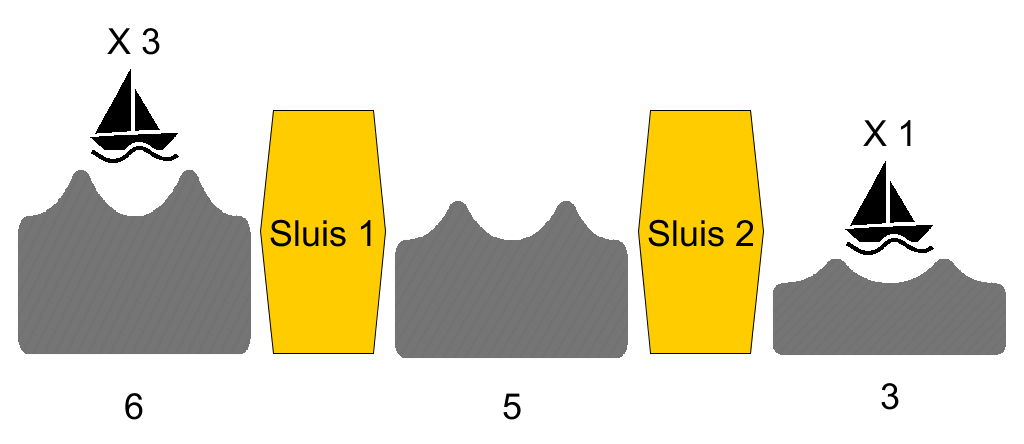
\includegraphics[width=\textwidth]{images/sluis_model.png}
    \caption{Model sluis dat twee sluisdeuren bevat en waterniveau bevat.}
	\label{fig:sluiceWaterLv}
\end{figure} \newline
\textbf{Waterpeil}\newline
Om het waterpeil te meten is er gekozen


\subsection{Ontwerpen}
//screen capture Uppaal model \newline

1) Waterniveau in sluiskolk gelijkmaken aan links \newline
2) Deuren links openen \newline
3) boten de sluiskolk in \newline
4a) opt: check of deuren dicht kunnen, geen obstructie \newline
4b) deuren links dicht \newline
5) waterniveau verlagen naar die van de rechter kant \newline
6) Deuren links openen \newline
7a) boten uit de sluiskolk \newline
7b) nieuwe boten van de rechter kant binnenlaten \newline
8a) opt: check of deuren dicht kunnen, geen obstructie \newline
8b) deuren rechts dicht \newline

Onderdelen templates: \newline
Sluisen \newline
Sensoren (water niveau) \newline
Actuatoren (licht, opt: geluid) \newline
Pompen


\subsection{Testen}

De kwaliteit van het gerelaiseerde model wordt gewaarborgd aan de hand van de functionaliteiten, beschreven onder '~\nameref{sec:FuncList}' op pagina ~\pageref{sec:FuncList}. Dit betekent dat er getest wordt op functionaliteit, daarnaast zullen ongewilde situaties zoals deadlocks (zie ~) en zeno gedrag (zie ~) onmogelijk gemaakt worden.

\section{Bijlagen}
\newpage
\bibliography{references}
\bibliographystyle{plain}


\end{document}


